\appendix{Представление графического материала}

Графический материал, выполненный на отдельных листах,
изображен на рисунках А.1--А.\arabic{числоПлакатов}.
\setcounter{числоПлакатов}{0}
\renewcommand{\thefigure}{А.\arabic{figure}} % шаблон номера для плакатов

\begin{landscape}

\begin{плакат}
    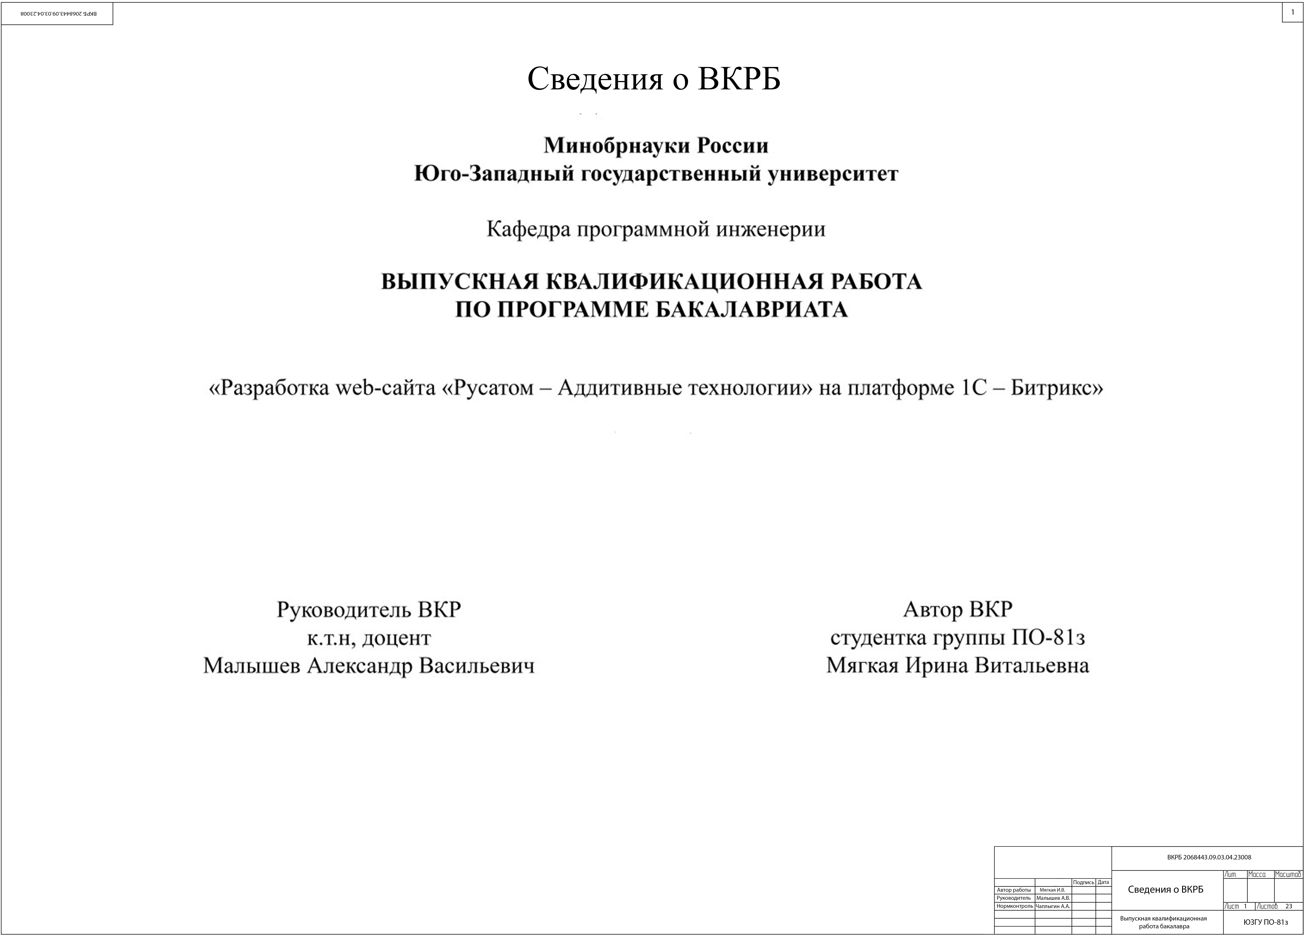
\includegraphics[width=0.81\linewidth]{плакат1}
    \заголовок{Сведения о ВКРБ}
    \label{pl1:image}      
\end{плакат}

\begin{плакат}
    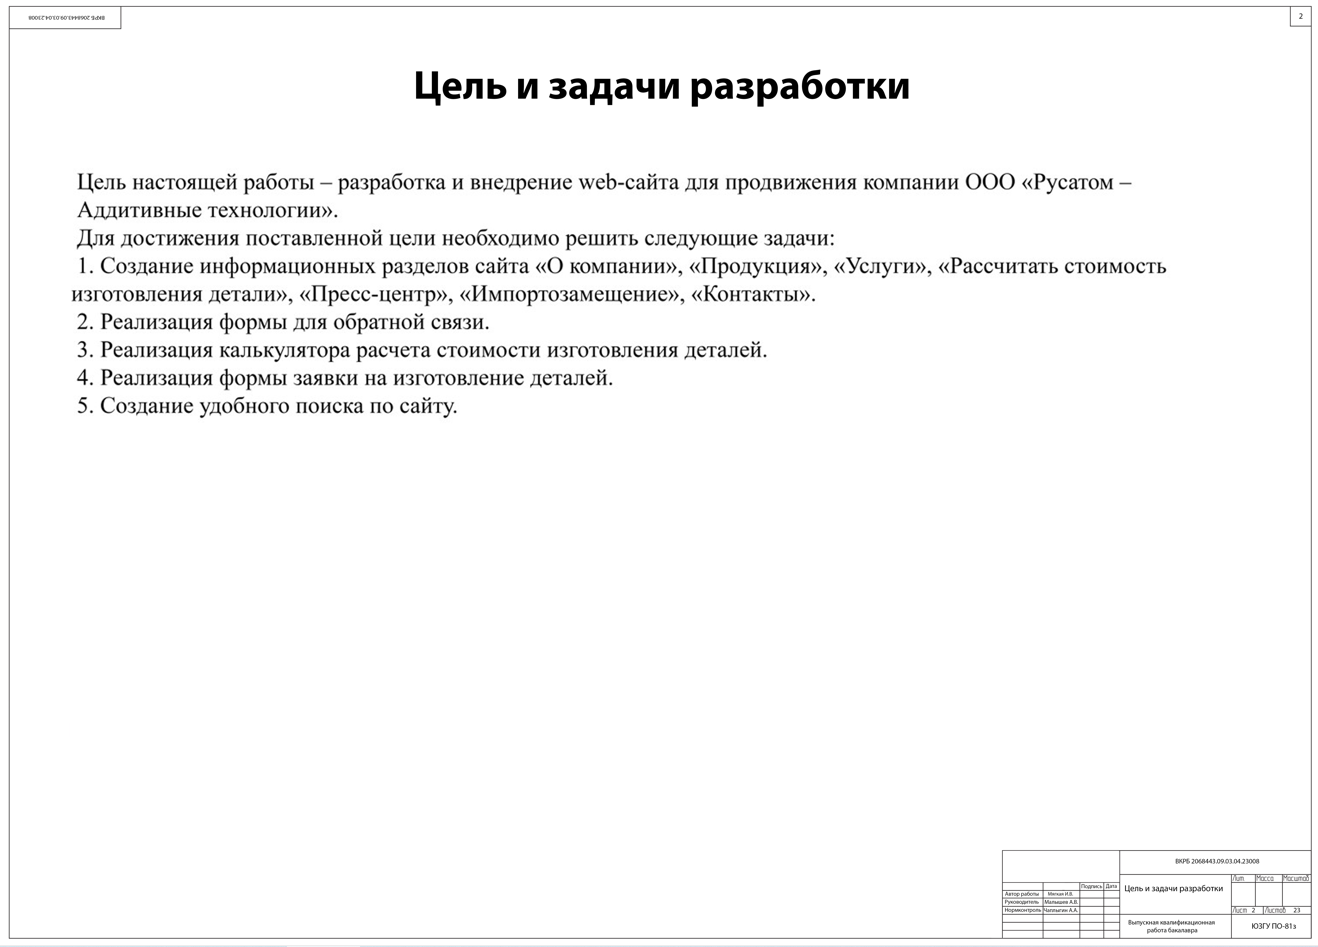
\includegraphics[width=0.82\linewidth]{плакат2}
    \заголовок{Цель и задачи разработки}
    \label{pl2:image}      
\end{плакат}

\begin{плакат}
    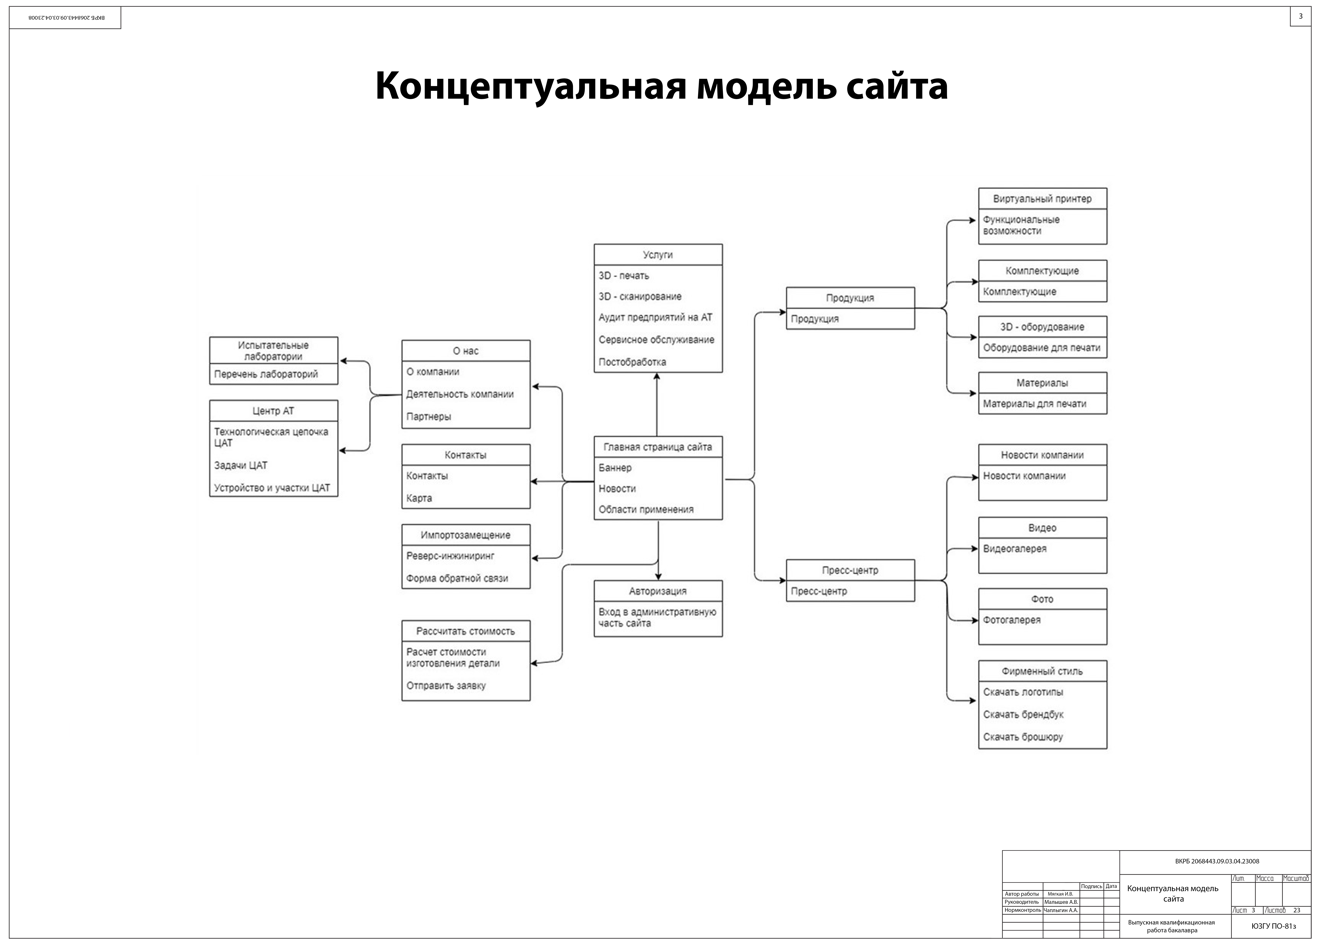
\includegraphics[width=0.82\linewidth]{плакат3}
    \заголовок{Концептуальная модель данных}
    \label{pl3:image}      
\end{плакат}

\begin{плакат}
    \includegraphics[width=0.82\linewidth]{плакат4}
    \заголовок{Диаграмма прецедентов}
    \label{pl4:image}      
\end{плакат}

\begin{плакат}
    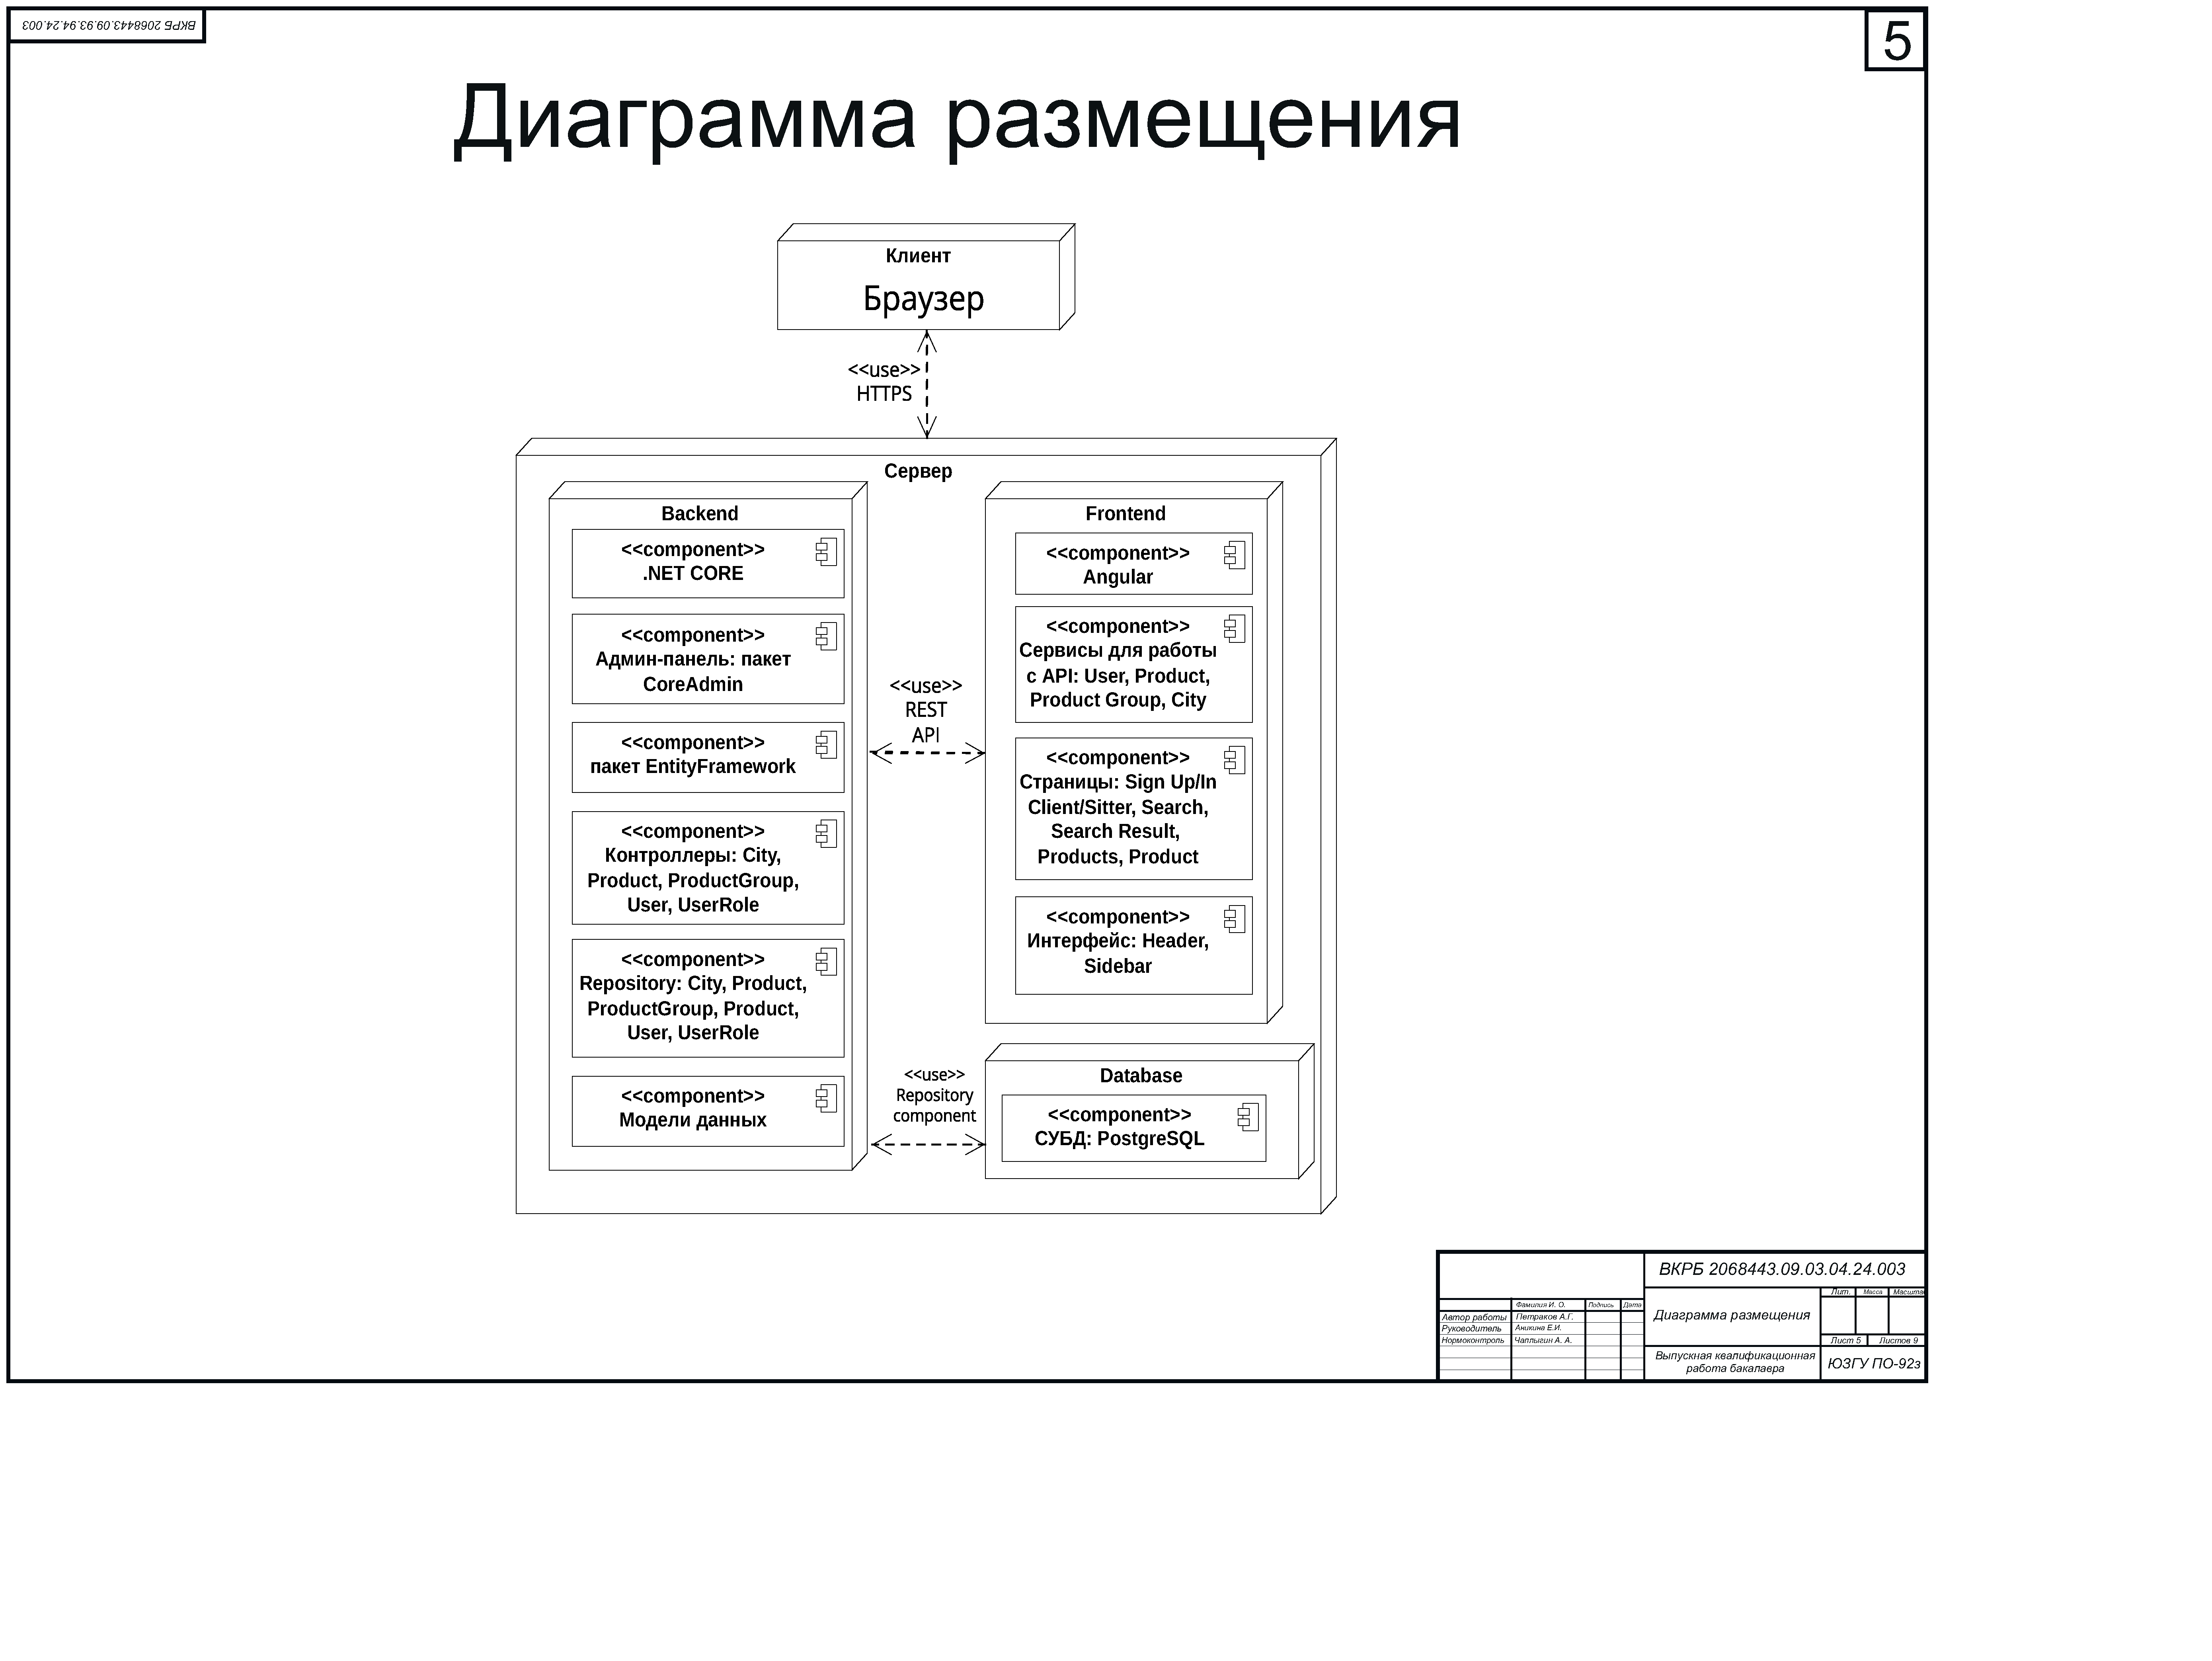
\includegraphics[width=0.82\linewidth]{плакат5}
    \заголовок{Диаграмма размещения}
    \label{pl5:image}
\end{плакат}

\begin{плакат}
    \includegraphics[width=0.82\linewidth]{плакат6}
    \заголовок{Регистрация}
    \label{pl6:image}
\end{плакат}

\begin{плакат}
    \includegraphics[width=0.82\linewidth]{плакат7}
    \заголовок{Поиск}
    \label{pl7:image}
\end{плакат}

\begin{плакат}
    \includegraphics[width=0.82\linewidth]{плакат8}
    \заголовок{Результаты поиска}
    \label{pl8:image}
\end{плакат}

\begin{плакат}
    \includegraphics[width=0.82\linewidth]{плакат9}
    \заголовок{Заключение}
    \label{pl9:image}
\end{плакат}

\end{landscape}
